\documentclass[10pt,twocolumn]{article}

\usepackage[margin=0.67in,columnsep=0.22in]{geometry}
\usepackage[T1]{fontenc}
\usepackage{lmodern}
\usepackage{microtype}
\usepackage{amsmath,amssymb,mathtools}
\usepackage{booktabs,tabularx,array,multirow}
\usepackage{enumitem}
\usepackage{xcolor}
\usepackage{hyperref}
\usepackage{url}
\usepackage{graphicx}
\usepackage{caption}
\usepackage{pgfplots}
\pgfplotsset{compat=1.18}
% Generated by experiments/synthesis/paper_numbers_v4.py. Do not edit by hand.
% source: results/holdout_v4/primary_endpoint_v4.json
% source: results/holdout_v4/secondary_endpoints_v4.json
% source: results/synthesis/boundary_synthesis_v4.json
% source: results/prop1/prop1_scoring_v4.json
\newcommand{\numAgInv}{0.913} % secondary.visibility.agreement.invariant.point
\newcommand{\numAgInvHi}{0.957} % secondary.visibility.agreement.invariant.ci[1]
\newcommand{\numAgInvLo}{0.913} % secondary.visibility.agreement.invariant.ci[0]
\newcommand{\numAgInvN}{21} % secondary agreement x 23
\newcommand{\numAgInvSmall}{22} % secondary.agreement_smallest_strength.invariant
\newcommand{\numAgSen}{0.632} % secondary.visibility.agreement.sensitive.point
\newcommand{\numAgSenHi}{0.684} % secondary.visibility.agreement.sensitive.ci[1]
\newcommand{\numAgSenLo}{0.579} % secondary.visibility.agreement.sensitive.ci[0]
\newcommand{\numAgSenN}{12} % secondary agreement x 19
\newcommand{\numAgSenSmall}{9} % secondary.agreement_smallest_strength.sensitive
\newcommand{\numCauseDesign}{1} % synthesis.cells cause=design
\newcommand{\numCauseMethod}{1} % synthesis.cells cause=method
\newcommand{\numCauseModel}{3} % synthesis.cells cause=model
\newcommand{\numCauseResources}{4} % synthesis.cells cause=resources
\newcommand{\numCertEfiveRzero}{0.422} % secondary.readout_certificate.P4b/E5.R0.unresolved
\newcommand{\numCertEfiveUnres}{0.867} % secondary.readout_certificate.P4b/E5.certificate.unresolved
\newcommand{\numCertEfourRzero}{0.509} % secondary.readout_certificate.P4a/E4.R0.unresolved
\newcommand{\numCertEfourUnres}{1.000} % secondary.readout_certificate.P4a/E4.certificate.unresolved
\newcommand{\numCovLoss}{0.418} % primary.main.coverage_loss_pooled
\newcommand{\numCovLossHi}{0.474} % secondary.coverage_pooled.R1.loss_ci[1]
\newcommand{\numCovLossLo}{0.360} % secondary.coverage_pooled.R1.loss_ci[0]
\newcommand{\numDevAgInv}{22} % synthesis.cells development==predicted, invariant
\newcommand{\numDevAgSen}{11} % synthesis.cells development==predicted, sensitive
\newcommand{\numDevHoldSame}{40} % synthesis.dev_holdout_label_agreement
\newcommand{\numEoneCerts}{0} % primary.per_structure.E1.R0_false_certifications
\newcommand{\numEoneCone}{0.015} % secondary.coverage.E1.C_R1
\newcommand{\numEoneCzero}{0.298} % secondary.coverage.E1.C_R0
\newcommand{\numEoneFCone}{0.0000} % primary.per_structure.E1.FC_R1
\newcommand{\numEoneFCzero}{0.0000} % primary.per_structure.E1.FC_R0
\newcommand{\numEoneFlipAlarm}{0.065} % secondary.flip_subset.E1.flipped.alarm_rate
\newcommand{\numEoneFlipped}{13} % secondary.flip_subset.E1.flipped_graphs
\newcommand{\numEoneGraphs}{0} % primary.per_structure.E1.R0_false_cert_graphs
\newcommand{\numEoneInter}{n/a} % secondary.coverage.E1.interception_R1
\newcommand{\numEoneNoFlipAlarm}{0.440} % secondary.flip_subset.E1.not_flipped.alarm_rate
\newcommand{\numEonePtwoInter}{n/a} % secondary.coverage.E1.interception_R1_P2
\newcommand{\numEthreeCerts}{36} % primary.per_structure.E3.R0_false_certifications
\newcommand{\numEthreeCone}{0.311} % secondary.coverage.E3.C_R1
\newcommand{\numEthreeCzero}{0.575} % secondary.coverage.E3.C_R0
\newcommand{\numEthreeFCone}{0.0000} % primary.per_structure.E3.FC_R1
\newcommand{\numEthreeFCzero}{0.0112} % primary.per_structure.E3.FC_R0
\newcommand{\numEthreeFlipAlarm}{0.625} % secondary.flip_subset.E3.flipped.alarm_rate
\newcommand{\numEthreeFlipped}{8} % secondary.flip_subset.E3.flipped_graphs
\newcommand{\numEthreeGraphs}{2} % primary.per_structure.E3.R0_false_cert_graphs
\newcommand{\numEthreeInter}{1.000} % secondary.coverage.E3.interception_R1
\newcommand{\numEthreeNoFlipAlarm}{0.380} % secondary.flip_subset.E3.not_flipped.alarm_rate
\newcommand{\numEthreePtwoInter}{0.222} % secondary.coverage.E3.interception_R1_P2
\newcommand{\numEtwoCerts}{195} % primary.per_structure.E2.R0_false_certifications
\newcommand{\numEtwoCone}{0.300} % secondary.coverage.E2.C_R1
\newcommand{\numEtwoCzero}{0.603} % secondary.coverage.E2.C_R0
\newcommand{\numEtwoFCone}{0.0159} % primary.per_structure.E2.FC_R1
\newcommand{\numEtwoFCzero}{0.0609} % primary.per_structure.E2.FC_R0
\newcommand{\numEtwoFlipAlarm}{0.472} % secondary.flip_subset.E2.flipped.alarm_rate
\newcommand{\numEtwoGraphs}{7} % primary.per_structure.E2.R0_false_cert_graphs
\newcommand{\numEtwoInter}{0.744} % secondary.coverage.E2.interception_R1
\newcommand{\numEtwoNoFlipAlarm}{0.429} % secondary.flip_subset.E2.not_flipped.alarm_rate
\newcommand{\numEtwoPtwoInter}{0.744} % secondary.coverage.E2.interception_R1_P2
\newcommand{\numFCGraphs}{9} % primary.per_structure sum of R0_false_cert_graphs
\newcommand{\numFCzero}{0.0103} % primary.main.FC_R0_pooled
\newcommand{\numFCzeroUp}{0.0179} % primary.main.FC_R0_upper_97.5
\newcommand{\numInterPooled}{0.784} % secondary.coverage_pooled.R1.interception
\newcommand{\numInterUnits}{231} % secondary.coverage_pooled.R1.interception_units
\newcommand{\numPfiveEonePower}{0.187} % secondary.cells.P5/E1.power
\newcommand{\numPfourbEfivePower}{0.010} % secondary.cells.P4b/E5.power
\newcommand{\numPoneEonePower}{0.40} % secondary.cells.P1/E1.power
\newcommand{\numPoneErrRaw}{0.145} % prop1.graphs mean error_rate_raw
\newcommand{\numPoneErrZne}{0.188} % prop1.graphs mean error_rate_zne
\newcommand{\numPoneHi}{0.548} % prop1.summary.wilson_95[1]
\newcommand{\numPoneHits}{45} % prop1.summary.hits
\newcommand{\numPoneLo}{0.356} % prop1.summary.wilson_95[0]
\newcommand{\numPoneRate}{0.45} % prop1.summary.hit_rate
\newcommand{\numPoneSep}{22} % prop1.by_reason.raw_separated.graphs
\newcommand{\numPoneTieZero}{42} % prop1.graphs: ties with zero errors
\newcommand{\numPoneTies}{47} % prop1.summary.ties
\newcommand{\numPoneUnc}{46} % prop1.by_reason.uncertified_raw_default.graphs
\newcommand{\numPoneUnr}{32} % prop1.by_reason.unresolved_anchor.graphs
\newcommand{\numPoneZneBetter}{8} % prop1.summary.zne_better_observed
\newcommand{\numPonebEone}{0.06} % synthesis.p1b.E1
\newcommand{\numPonebEthree}{0.76} % synthesis.p1b.E3
\newcommand{\numPthreeEthreePower}{0.38} % secondary.cells.P3/E3.power
\newcommand{\numPtwoEfpFA}{0.133} % secondary.cells.P2/E5'.false_alarm
\newcommand{\numPtwoEfpPower}{0.132} % secondary.cells.P2/E5'.power
\newcommand{\numPtwoInter}{0.662} % secondary.coverage_pooled.R1_P2.interception
\newcommand{\numPtwoLoss}{0.142} % secondary.coverage_pooled.R1_P2.loss
\newcommand{\numPtwoLossHi}{0.173} % secondary.coverage_pooled.R1_P2.loss_ci[1]
\newcommand{\numPtwoLossLo}{0.111} % secondary.coverage_pooled.R1_P2.loss_ci[0]
\newcommand{\numPtwodFC}{+0.0067} % primary.P2.dFC
\newcommand{\numPtwodFChi}{+0.0118} % primary.P2.dFC_upper_97.5
\newcommand{\numPtwodFClo}{+0.0021} % primary.P2.dFC_lower_2.5
\newcommand{\numdFC}{+0.0080} % primary.main.dFC
\newcommand{\numdFChi}{+0.0142} % primary.main.dFC_upper_97.5
\newcommand{\numdFClo}{+0.0029} % primary.main.dFC_lower_2.5

% Generated by experiments/synthesis/hw_paper_v4_1.py. Do not edit by hand.
\newcommand{\numEfiveRatio}{0.28} % protocol v4 E5: tau 0.01 / c*(0.1, 0.1)
\newcommand{\numEfiveRho}{0.11} % protocol v4 E5: tau 0.01 / (0.1 x 0.9)
\newcommand{\numHwCiExcl}{6} % pair-preparations whose unadjusted 95% interval for c excludes 0
\newcommand{\numHwDetRej}{0} % analysis.detection_rejections
\newcommand{\numHwMainSec}{48} % raw/main_job0.usage_seconds
\newcommand{\numHwMaxRatio}{0.023} % max c_hat/c* over pair-preparations
\newcommand{\numHwMaxRho}{0.011} % max |rho_hat| over pair-preparations
\newcommand{\numHwMaxUpperRatio}{0.043} % max (95% upper bound of c)/c*
\newcommand{\numHwMedianErr}{1.71} % run_manifest.median_readout_error (percent)
\newcommand{\numHwMinDetHolm}{0.15} % min Holm-adjusted detection p
\newcommand{\numHwPilotSec}{3} % raw/pilot_job0.usage_seconds
\newcommand{\numHwRelRej}{0} % analysis.relevance_rejections
\newcommand{\numHwShots}{87,200} % analysis.shots_per_circuit
\newcommand{\numHwSmin}{10,000} % allocation.s_min
\newcommand{\numHwTests}{56} % analysis.m_tests_per_family
\newcommand{\numHwTotalSec}{51} % pilot + main usage_seconds


\definecolor{linkblue}{RGB}{28,78,121}
\hypersetup{colorlinks=true,allcolors=linkblue,pdfauthor={Zhen-Jun Liu},
  pdftitle={Runtime Visibility Limits of Bias Probes for Quantum Error-Mitigated Selection}}
\captionsetup{font=small,labelfont=bf,skip=4pt}
\setlist{nosep,leftmargin=*}
\setlength{\parindent}{0.8em}
\setlength{\parskip}{0pt}
\setlength{\tabcolsep}{4pt}
\renewcommand{\arraystretch}{1.12}
\newcommand{\E}{\mathbb{E}}
\newcommand{\Prb}{\mathbb{P}}
\newcommand{\ind}{\mathbb{1}}
\newcommand{\code}[1]{\texttt{#1}}
\newcommand{\grp}[1]{\multicolumn{3}{@{}l}{\textit{#1}}\\}

\title{\textbf{Runtime Visibility Limits of Bias Probes for\\
Quantum Error-Mitigated Selection}\vspace{0.35em}\\
\large A Preregistered Fixed-Budget Study}
\author{Zhen-Jun Liu}
\date{19 November 2026 (v4.2; v4.0 is release v1.0 and v4.1 is release v1.1)}

\begin{document}
\maketitle

\begin{abstract}
A confidence interval controls sampling error but not differential systematic
bias, so a quantum computation can select the wrong candidate with high
reported confidence. We ask when a runtime bias probe, paid for out of the same
fixed shot budget, can catch such a wrong but confident selection. In a
preregistered study of QAOA--MaxCut top-1 decisions, six probes were tested
against seven gate and readout error structures, and a single holdout
was run once in noisy simulation. Reserving a tenth of the shots for a
structure-matched probe and abstaining on alarm lowered the pooled
false-certification rate by $\numdFC$, the registered ``improvement'' outcome,
but at a coverage loss of $\numCovLoss$, and the gain came only from two
coherent gate errors. A registered test of when zero-noise extrapolation beats
raw estimation scored $\numPoneHits$ of 100 hits. Probe visibility is
therefore mechanism-specific and costly: a probe helps only where an error both
reverses decisions and leaves a signature the probe can resolve within its
share of the budget. An exploratory hardware test, registered afterwards, found
readout correlations on one IBM Quantum device far below the level at which
tensored readout mitigation fails.
\end{abstract}

\section{Introduction}

Selection tasks need the sign of a contrast, not an accurate estimate. Quantum
error mitigation (QEM) spends extra circuits, shots, or model assumptions to
reduce estimator error without full fault
tolerance\cite{temme2017,li2017,endo2018,endo2021jpsj,cai2023}, and it is
usually judged by bias, variance, or mean-squared error. When two candidates
acquire different systematic biases, however, a more accurate average need not
yield a more reliable choice.

Known sampling-cost bounds concern estimators, and this study concerns
decisions. For broad classes of protocols and noise models, the samples needed
for a fixed estimator accuracy grow exponentially with circuit
depth\cite{takagi2022,takagi2023,tsubouchi2023}, and worst-case noisy circuits
can need superpolynomially many samples already at shallow
depth\cite{quek2024}. We work at small scale, where mitigation overhead is
modest, and ask a complementary question: can a decision certified by a
confidence interval be recognized as wrong at runtime?

Let the ideal candidate values be $\mu_A$ and $\mu_B$, with ideal gap
$g=\mu_A-\mu_B$ and margin $\Delta=|g|$. If noise adds biases $b_A$ and $b_B$,
the decision-relevant bias is
\begin{equation}
  \beta=(b_A-b_B)\operatorname{sign}(g),
  \label{eq:beta}
\end{equation}
and the ideal decision is reversed whenever $\Delta+\beta<0$. A narrow interval
can then exclude zero and still certify the wrong sign, because it controls
finite-shot variation around a biased center.

A useful probe must pass three tests: it must respond to the harmful direction,
keep enough power at its shot share, and intercept enough wrong certifications
to repay the target shots it consumes. A probe that fails the first test is
blind in principle, one that fails the second is visible only in the population
limit, and one that fails the third can be informative yet harm the deployed
decision rule.

\paragraph{Contributions.}
\begin{itemize}
\item A preregistered map of which runtime probes can see which error
  structures under one fixed budget, with analytically invariant cells
  reported separately from budget-sensitive ones (Section~\ref{sec:results}).
\item An exact condition, free of distributional assumptions, for when
  spending shots on a probe lowers the wrong-decision rate
  (Eq.~\eqref{eq:worth}), and a confirmatory test of it on a 100-graph holdout.
\item A registered, falsifiable test of when zero-noise extrapolation should
  beat raw estimation, and a registered hardware check of the readout
  structures used in simulation.
\end{itemize}
Null, negative, and mismatched outcomes were admissible under the registration
and are reported as such.

\section{Related work}\label{sec:related}

\paragraph{Mitigation methods.} Zero-noise extrapolation amplifies noise and
extrapolates to zero\cite{temme2017,li2017}, by digital gate
folding\cite{giurgica2020} or identity insertion\cite{he2020}, and has been
demonstrated on superconducting
hardware\cite{kandala2019,kim2023natphys,kim2023}. Probabilistic error
cancellation inverts a learned noise model at a sampling
cost\cite{temme2017,endo2018,vandenberg2023}. Symmetry verification discards
or corrects outcomes that violate a conserved
quantity\cite{bonetmonroig2018,mcardle2019,sagastizabal2019}, and virtual
distillation suppresses noise with several copies of a state\cite{huggins2021}.
Clifford data regression learns a correction from classically simulable
circuits\cite{czarnik2021,lowe2021,strikis2021}. Readout mitigation ranges from
detector tomography\cite{maciejewski2020,chen2019detector} and tensored or
subspace inversion\cite{bravyi2021,nation2021} to correlated-readout
models\cite{maciejewski2021}, twirled readout\cite{vandenberg2022trex}, and
readout rebalancing\cite{hicks2021}. Randomized compiling converts coherent
errors into stochastic Pauli
noise\cite{knill2005,wallman2016,hashim2021}. Each of our probes borrows one of
these mechanisms, but uses it to detect bias rather than to correct it.

\paragraph{Limits of mitigation.} Beyond the estimator-level cost bounds cited
above\cite{takagi2022,takagi2023,tsubouchi2023,quek2024}, noise limits what
variational and optimization algorithms can
achieve\cite{stilckfranca2021,wang2021nibp}. These results bound how much
accuracy mitigation can buy; they do not say whether a given decision is
right.

\paragraph{Evaluating mitigation.} Benchmarks compare mitigation methods across
circuit sizes\cite{cirstoiu2023} or at a common shot budget\cite{bultrini2023},
and recent audits show how parameter choices and device drift can create
apparent improvements in zero-noise
extrapolation\cite{koster2026,koster2026claim}. Other work quantifies
finite-shot uncertainty to tune mitigation
hyperparameters\cite{prodius2026}, derives finite-shot operating windows for
specific estimators\cite{scavino2026pec,scavinoalfaro2026windows}, or bounds
the systematic error caused by violation of the assumed noise
model\cite{govia2025}. Closest to this study, decision-kernel theory shows
that a gap-based decision depends only on the distribution of the residual
gap, separates common-mode from differential bias under a fixed total budget,
and gives a local identifiability condition\cite{scavino2026}. We add runtime
probes that try to observe the differential bias itself, a global sign
criterion for blindness (Appendix~\ref{app:local}), and a confirmatory test.

\paragraph{Characterization and identifiability.} Randomized benchmarking and
its variants compress noise into average error
rates\cite{magesan2011,gambetta2012,erhard2019,proctor2022mirror,proctor2022capabilities},
and average fidelity can understate the worst-case error, most strongly for
coherent errors\cite{kueng2016,sanders2016}.
Pauli channels can be estimated efficiently\cite{flammia2020pauli}, but part of
Pauli noise on Clifford gates is provably unlearnable\cite{chen2023learnability},
gate set tomography carries a gauge freedom\cite{nielsen2021gst}, and the
Pauli twirling approximation has been studied as an effective error
model\cite{geller2013}. Crosstalk can be
detected through conditional dependence of outcomes\cite{sarovar2020}.
Certification frames these questions as hypothesis tests\cite{eisert2020,kliesch2021}.
Our blindness lemma states the same kind of limit for a decision.

\paragraph{Statistical decision theory.} Partial identification studies what
can be learned when observations define a set rather than a
point\cite{imbens2004,tamer2010}. Negative controls reveal bias when the
control shares the target's unmeasured causes\cite{lipsitch2010}; our probes
are an analogy to this condition, not an instance of it. Sensitivity analysis
asks how large a hidden bias must be to overturn a
conclusion\cite{rosenbaum1987,vanderweele2017}, and honest intervals widen by
a worst-case bias fixed in advance\cite{armstrong2020}. Ranking and selection
and best-arm identification allocate samples to find the best
candidate\cite{bechhofer1954,kimnelson2006,chen2000ocba,kaufmann2016,garivier2016};
under model misspecification such guarantees can fail\cite{ghosh2017}. We use
a fixed, non-sequential budget; sequential tests and confidence
sequences\cite{wald1945,howard2021} are left to future work, and the
registration practice follows Ref.~\cite{nosek2018}.

\section{Problem and methods}

\subsection{Decision, identification, and visibility}

For QAOA--MaxCut\cite{farhi2014,zhou2020qaoa,harrigan2021}, a bit string $z$ on
graph $G=(V,E)$ receives the normalized score
\begin{equation}
  s_G(z)=\frac{1}{|E|}\sum_{(i,j)\in E}\ind\{z_i\neq z_j\}\in[0,1].
\end{equation}
Each graph has two frozen candidate parameter vectors; their expected scores
define $g$, and the sign of an observed gap selects a candidate.

Let $D$ denote all target and probe observations and $\mathcal M(D)$ the
admissible error mechanisms compatible with them. The identification region
for the ideal gap is
\begin{equation}
  \mathcal I_g(D)=\{g(M):M\in\mathcal M(D)\}.
  \label{eq:idregion}
\end{equation}
If it contains both positive and non-positive values, the decision is not
sign-identified. This is a population concept, distinct from a confidence
interval for shot noise; we use it to state blindness, not to optimize
Eq.~\eqref{eq:idregion} for every cell.

For each probe--structure cell the protocol freezes a statistic and a matched
null. A cell is \emph{invariant} if the population statistic is identical under
the structure and its null, so no threshold can recover power, and
\emph{sensitive} if a nonzero population contrast exists but may be
underpowered at the frozen budget. The visible/partial/blind label combines
this analytic relation with frozen power and false-alarm rules, and the two
strata are always reported separately.

\subsection{Probes}

Each probe targets one projection of the error process
(Table~\ref{tab:probes}); none is an omnibus detector. Positive-cost probes
take $n_P=1{,}638$ of the $N=16{,}384$ shots and leave $n_T=14{,}746$ for the
targets; P5 reuses target counts at no cost. P0, the target-only interval
comparator, is not a probe and is excluded from the visibility matrix.

\begin{table}[t]
\centering
\caption{Six probes, each aimed at one error mechanism.}
\label{tab:probes}
\small
\begin{tabularx}{\columnwidth}{@{}lXl@{}}
\toprule
Probe & Statistic & Aimed at \\
\midrule
P1 & Gap change under unitary folding (scales 1, 3) & Gate-count noise \\
P2 & Observed vs ideal gap of a Clifford twin & Transferable gate bias \\
P3 & Gap change under 16 Pauli frames & Coherent two-qubit error \\
P4a & Assignment deviation, all-0/all-1 inputs & Readout marginals, drift \\
P4b & One component from pair preparations & Pair readout correlation \\
P5 & Bit-complement asymmetry of target counts & Symmetry breaking \\
\bottomrule
\end{tabularx}
\end{table}

Thresholds are matched-null quantiles. Within each width--depth stratum, the
development null scores $T_{(1)}\le\cdots\le T_{(n)}$ give
\begin{equation}
  \tau=T_{\min\{n,\lceil(n+1)(1-\alpha)\rceil\}},\qquad \alpha=0.05,
\end{equation}
and a probe alarms when $T>\tau$. Decision endpoints instead calibrate alarms
on the clean structure E0, as a deployed rule would without knowing the active
error, so no structure-specific information leaks into the operational rule.

\subsection{Fixed-budget decision rules}\label{sec:rules}

Rule R0 certifies when the target gap interval excludes zero. Rule R1 gives 10\%
of the budget to the structure-designated probe and certifies only when the
interval excludes zero and the probe does not alarm. With $W_f$ the event that
the reduced-shot decision is wrong and $A_f$ the alarm, let
\begin{equation}
  q_f=\Prb(W_f),\quad d_f=\Prb(A_f\cap W_f),\quad R_f=q_f-d_f.
\end{equation}
Against the all-target error probability $q_0$, the probe lowers the
wrong-decision risk if and only if
\begin{equation}
  d_f>q_f-q_0.
  \label{eq:worth}
\end{equation}
The left side is useful interception and the right side the cost of the
removed target shots. Equation~\eqref{eq:worth} is exact for an abstaining rule
and assumes no independence (Appendix~\ref{app:prop2}). Because abstaining
mechanically removes errors, false certification and coverage are reported
separately rather than merged into a post hoc loss.

\section{Experimental design}

\subsection{Graphs, candidates, and error structures}

The holdout has 100 graphs, four per width--depth stratum (widths 4--8, depths
1--5), drawn from Erd\H{o}s--R\'enyi, Watts--Strogatz, and Barab\'asi--Albert
families. Each graph has two frozen QAOA candidates, compiled with
Qiskit\cite{javadiabhari2024} to \code{rz,sx,x,cx} without routing or
optimization; one candidate carries a logically cancelling CX--CX pair after
each cost layer, a frozen gate-count contrast that leaves its ideal unitary
unchanged. Noisy outcome probabilities are computed exactly by the project's
own state-vector and density-matrix code, and shots are sampled from them.

\begin{table}[t]
\centering
\caption{Seven error structures. Each matched null keeps the baseline and
zeroes only the tested component; full grids are in
Table~\ref{tab:grids}.}
\label{tab:errors}
\small
\begin{tabularx}{\columnwidth}{@{}lXl@{}}
\toprule
Code & Mechanism & Strength \\
\midrule
E1 & Two-qubit depolarizing after each CX & $p\le0.04$ \\
E2 & Over-rotation of cost $R_Z$ gates & $|\epsilon|\le0.04$ \\
E3 & Coherent $ZZ$ crosstalk after each CX & $|\zeta|\le0.04$ \\
E4 & Independent asymmetric readout & rates $\le0.12$ \\
E5 & Correlated pair readout flips & $|\tau|\le0.01$ \\
E5$'$ & Three-body readout flips (synthetic) & $|\tau|\le0.0156$ \\
E6 & Readout drift over eight blocks & $|\delta|\le0.03$ \\
\bottomrule
\end{tabularx}
\end{table}

Matched nulls repair a defect of protocol v3. E5 and E5$'$ keep their
independent marginal flips in the null and E6 keeps its baseline assignment
rates, so a probe cannot score visibility by reacting to the baseline. The
clean structure E0 adds equal offsets to both candidates and cannot change a
decision. E7, fake-backend snapshots, and probe combinations are exploratory
and outside the primary matrix.

\subsection{Registered matrix and endpoints}

The registered matrix predicts blindness for most cells
(Table~\ref{tab:matrix}). All invariant cells are predicted blind; the
sensitive stratum holds every non-blind prediction and two blind ones, P1/E6
and P3/E6, whose small contrast is predicted to stay below the power boundary.

\begin{table}[t]
\centering
\caption{Registered predictions for the 42 probe--structure cells.}
\label{tab:matrix}
\small
\begin{tabular}{@{}lrrrr@{}}
\toprule
Stratum & Visible & Partial & Blind & Total \\
\midrule
Invariant & 0 & 0 & 23 & 23 \\
Sensitive & 4 & 13 & 2 & 19 \\
\midrule
Total & 4 & 13 & 25 & 42 \\
\bottomrule
\end{tabular}
\end{table}

The primary estimand is the mean reduction in false certification, that is,
certifying the wrong ideal winner, over the seven structures:
\begin{equation}
 \Delta_{\rm FC}=\frac{1}{7}\sum_{s=1}^{7}
 \{\mathrm{FC}_s(R0)-\mathrm{FC}_s(R1)\}.
 \label{eq:dfc}
\end{equation}
Its 95\% interval comes from 10,000 stratified graph-cluster bootstrap
resamples, which resample whole graphs\cite{field2007} with indices shared
across rules and structures. The registered outcome is ``improvement'' if the
lower endpoint is positive, ``no decision problem'' if the 97.5th percentile of
pooled R0 false certification is below 0.01, and ``inconclusive'' otherwise.
Secondary endpoints are coverage loss, interception, alarms on flipped graphs,
a structure-agnostic P2 rule, visibility agreement per stratum, and a readout
certificate that applies only where the probe measures the modeled readout
component.

\subsection{Registration and reproducibility}

Public OSF records fix the order of events (Appendix~\ref{app:chron}):
protocol v4 with its execution code before any noisy data, a confirmatory lock
of the development thresholds before the holdout existed, the Proposition-1
predictions before their scoring split, and the hardware amendment before any
hardware data. Every random stream derives from one NumPy \code{SeedSequence}
key; raw and failed rows are append-only, every reported number is recomputed
from them, and the holdout and Proposition-1 scoring each refuse a second run.

\section{Results}\label{sec:results}

All results are noisy simulation on the holdout, read once, except the analytic
result below and the hardware addendum. Table~\ref{tab:results} collects the
registered estimates; the text refers to it rather than repeating them.

\begin{table}[t]
\centering
\caption{Registered results. Intervals are 95\% graph-cluster bootstrap
intervals unless marked W (Wilson score interval\cite{wilson1927}); ``upper'' is a one-sided 95\% bound
(97.5th percentile for R0 FC). FC, false certification.}
\label{tab:results}
\small
\begin{tabular}{@{}lll@{}}
\toprule
Quantity & Estimate & 95\% interval \\
\midrule
\grp{Primary: designated probe (R1 vs R0)}
$\Delta_{\rm FC}$ & $\numdFC$ & $[\numdFClo,\numdFChi]$ \\
R0 FC, pooled & $\numFCzero$ & upper $\numFCzeroUp$ \\
Coverage loss & $\numCovLoss$ & $[\numCovLossLo,\numCovLossHi]$ \\
Interception & $\numInterPooled$ & \\
Graphs with R0 FC & $\numFCGraphs$/100 & \\
\midrule
\grp{Secondary: P2 for every structure}
$\Delta_{\rm FC}$ & $\numPtwodFC$ & $[\numPtwodFClo,\numPtwodFChi]$ \\
Coverage loss & $\numPtwoLoss$ & $[\numPtwoLossLo,\numPtwoLossHi]$ \\
Interception & $\numPtwoInter$ & \\
\midrule
\grp{Secondary: agreement with registered labels}
Invariant cells & $\numAgInvN$/23 & $[\numAgInvLo,\numAgInvHi]$ \\
Sensitive cells & $\numAgSenN$/19 & $[\numAgSenLo,\numAgSenHi]$ \\
\midrule
\grp{Secondary: readout certificate, unresolved}
P4a/E4: cert.\ / R0 & $\numCertEfourUnres$ / $\numCertEfourRzero$ & \\
P4b/E5: cert.\ / R0 & $\numCertEfiveUnres$ / $\numCertEfiveRzero$ & \\
\midrule
\grp{Secondary: Proposition-1 prediction test}
Hits & $\numPoneHits$/100 & $[\numPoneLo,\numPoneHi]$ W \\
Misses: ties / ZNE better & $\numPoneTies$ / $\numPoneZneBetter$ & \\
Mean error: raw / ZNE & $\numPoneErrRaw$ / $\numPoneErrZne$ & \\
\midrule
\grp{Exploratory: hardware, \numHwTests{} pair-preparations}
Rejections: rel.\ / det.\ & $\numHwRelRej$ / $\numHwDetRej$ & \\
Max $|\hat\rho|$ (E5 level) & $\numHwMaxRho$ ($\numEfiveRho$) & \\
Max $\hat c/c^\ast$ (E5 level) & $\numHwMaxRatio$ ($\numEfiveRatio$) & upper $\numHwMaxUpperRatio$ \\
\bottomrule
\end{tabular}
\end{table}

\subsection{Uniform readout cannot reverse a decision}

Uniform readout noise shrinks a QAOA gap but never flips it. Under the frozen
ideal model, QAOA--MaxCut has global bit-complement symmetry, so
$\langle Z_i\rangle=0$. For uniform independent assignment noise with
$\widetilde Z_i=\lambda Z_i+\delta$, each edge contrast scales by $\lambda^2$:
\begin{equation}
  g_{\rm noisy}=\lambda^2 g,\qquad
  \frac{\beta}{\Delta}=-(1-\lambda^2)\in(-1,0].
  \label{eq:readoutscale}
\end{equation}
The same bound holds for the frozen E6 mixture. This limits the decision-flip
evidence that E4 and E6 can supply; it does not make their probes useless for
detecting readout change. Design checks, the pre-data defect audit, and the
development results are summarized in Appendix~\ref{app:design}.

\subsection{Primary endpoint: a real but costly improvement}

The registered outcome is \emph{improvement}: the interval for $\Delta_{\rm FC}$
excludes zero (Table~\ref{tab:results}). A decision problem exists at this
budget, since pooled R0 false certification exceeds the 0.01 bound, and the
outcome is unchanged when that bound is set to 0.005 or 0.02.

The gain comes entirely from the two coherent gate errors
(Table~\ref{tab:primary}). Under E2 and E3, R1 intercepted most or all of R0's
false certifications, which were concentrated in a few graphs. Under the other
five structures R0 never false-certified, so there was nothing to intercept.
The price is coverage: R1 never certified under the readout structures, because
P4a's clean-E0 threshold is zero and every readout flip alarms, and it almost
never certified under E1.

\begin{table*}[t]
\centering
\caption{The improvement comes from E2 and E3 and is bought with coverage. FC,
false certification rate; C, coverage; Int., share of R0 false certifications
that R1 does not certify. Alarm rates compare graphs whose noisy population gap
reverses the ideal decision with all others. E4--E6 (no false certification by
either rule; R1 coverage 0) are omitted.}
\label{tab:primary}
\small
\begin{tabular}{@{}llrrrrrrrrr@{}}
\toprule
 & & \multicolumn{2}{c}{R0 false certifications} & \multicolumn{2}{c}{FC} & \multicolumn{2}{c}{C} & & \multicolumn{2}{c}{Alarm rate} \\
\cmidrule(lr){3-4}\cmidrule(lr){5-6}\cmidrule(lr){7-8}\cmidrule(l){10-11}
Structure & Probe & runs & graphs & R0 & R1 & R0 & R1 & Int. & flipped & other \\
\midrule
E1 depolarizing & P1 & $\numEoneCerts$ & $\numEoneGraphs$ & $\numEoneFCzero$ & $\numEoneFCone$ & $\numEoneCzero$ & $\numEoneCone$ & -- & $\numEoneFlipAlarm$ & $\numEoneNoFlipAlarm$ \\
E2 over-rotation & P2 & $\numEtwoCerts$ & $\numEtwoGraphs$ & $\numEtwoFCzero$ & $\numEtwoFCone$ & $\numEtwoCzero$ & $\numEtwoCone$ & $\numEtwoInter$ & $\numEtwoFlipAlarm$ & $\numEtwoNoFlipAlarm$ \\
E3 $ZZ$ crosstalk & P3 & $\numEthreeCerts$ & $\numEthreeGraphs$ & $\numEthreeFCzero$ & $\numEthreeFCone$ & $\numEthreeCzero$ & $\numEthreeCone$ & $\numEthreeInter$ & $\numEthreeFlipAlarm$ & $\numEthreeNoFlipAlarm$ \\
\bottomrule
\end{tabular}
\end{table*}

\subsection{Secondary endpoints}

\paragraph{One structure-agnostic probe trades better.} Using P2 for every
structure also improved false certification, at about a third of the coverage
loss of the designated probes (Table~\ref{tab:results}). It intercepted the
same E2 false certifications but few under E3.

\paragraph{Alarms track decision flips only for E3.} P3 alarmed more often on
E3 graphs whose decision was flipped than on the others, P2 under E2 hardly
discriminated, and P1 under E1 alarmed least where the decision was wrong in
the population (Table~\ref{tab:primary}), although R0 never certified those
graphs.

\paragraph{Most predicted blind cells were blind.} Agreement with the
registered labels was high in the invariant stratum and moderate in the
sensitive one (Table~\ref{tab:results}; Fig.~\ref{fig:map}). The two invariant
disagreements are P5/E1, investigated before the lock
(Appendix~\ref{app:design}), and P2/E5$'$, whose alarm rate equals its
matched-null rate: a threshold-transfer failure, not a response to the
structure.

\begin{figure*}[t]
\centering
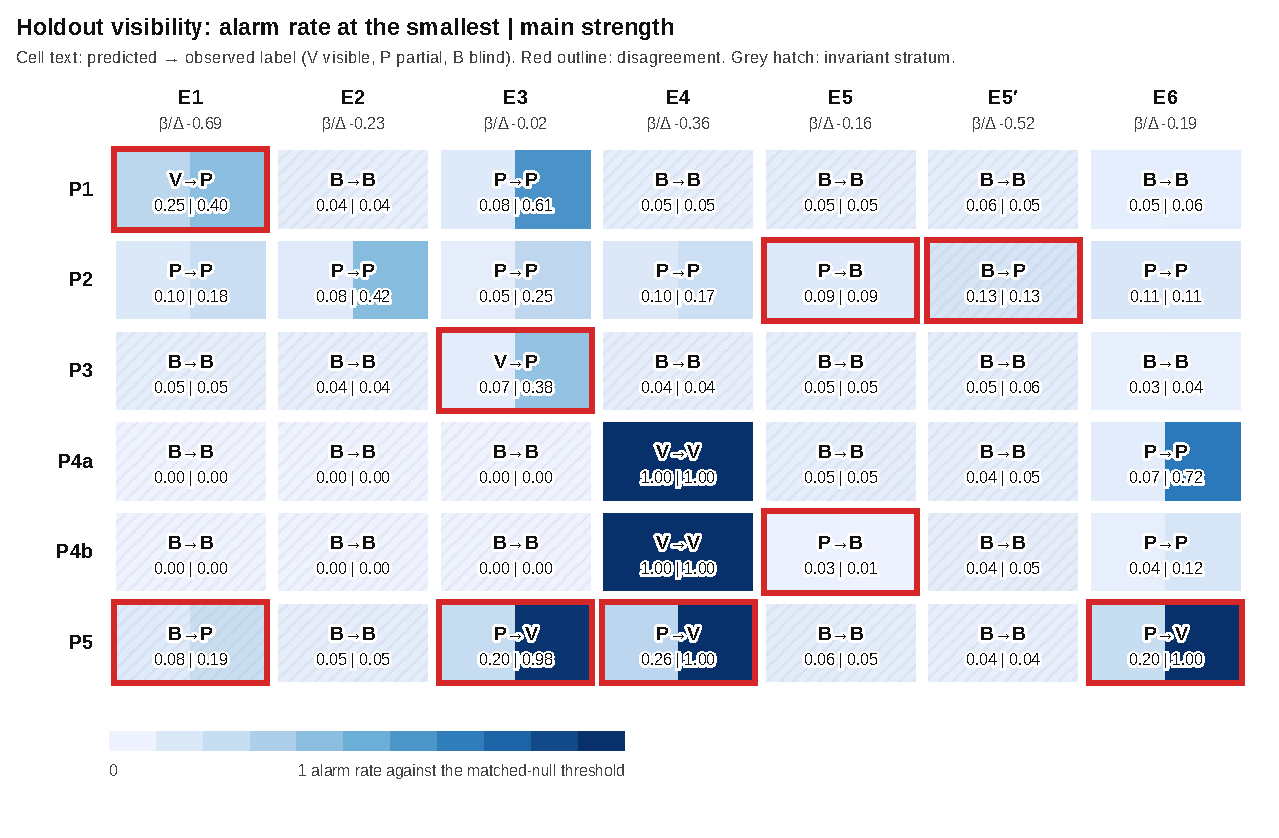
\includegraphics[width=\textwidth]{../figures/boundary_map_v4.pdf}
\caption{\textbf{Most cells stay blind as predicted; readout probes see
readout structures, the symmetry probe sees symmetry-breaking ones, and
disagreements concentrate in the budget-sensitive stratum.} Each cell gives the
holdout alarm rate against the matched-null threshold at the smallest (left)
and main (right) frozen strength, with predicted$\to$observed labels. Red
outlines mark disagreements; hatching marks the invariant stratum. Column
headers give the median $\beta/\Delta$ at the main point over the 100 holdout
graphs.}
\label{fig:map}
\end{figure*}

\paragraph{The readout certificate gives no benefit at this budget.} Requiring
the target to clear a bound over all readout channels consistent with the
probe intervals left nearly every run unresolved, and neither rule
false-certified. P4b spreads its shots over $4\binom{w}{2}$ circuits, so its
simultaneous intervals stay wide.

\paragraph{The probe-fraction endpoint was not evaluable.} Thresholds were
calibrated only at a 10\% probe share; calibrating others after the lock would
have changed the registered rule.

\subsection{Why predictions failed (exploratory)}

Each disagreement received one cause by a fixed rule
(Table~\ref{tab:causes}; Appendix~\ref{app:causes}). Most were resource
failures, in which a real contrast was underpowered at the probe budget, or
conservative model errors, in which P5 saw more than predicted. At the decision
level, the zero readout coverage of R1 and the unevaluable probe fraction are
design consequences, and the unresolved certificate is a resource consequence.

\begin{table}[t]
\centering
\caption{Causes of the holdout disagreements, assigned mechanically.}
\label{tab:causes}
\small
\begin{tabularx}{\columnwidth}{@{}lXr@{}}
\toprule
Cause & Cells & $n$ \\
\midrule
Resources & P1/E1, P3/E3 (pred.\ visible); P2/E5, P4b/E5 (pred.\ partial) & $\numCauseResources$ \\
Model & P5/E3, P5/E4, P5/E6 & $\numCauseModel$ \\
Method & P5/E1 & $\numCauseMethod$ \\
Design & P2/E5$'$ & $\numCauseDesign$ \\
\bottomrule
\end{tabularx}
\end{table}

\subsection{Proposition-1 prediction test}

The registered rule never predicted that zero-noise extrapolation would win,
so the test could not assess recognition of ZNE-favourable graphs. For each
holdout graph identity, a pilot (split 30) with four QAOA candidates under E1
depolarizing noise ($p=0.04$) predicted whether raw estimation or linear ZNE
would give lower top-1 error on separate scoring data (split 31) at equal
budget. It predicted raw for all 100 graphs, and ties counted as misses
(Table~\ref{tab:results}). Most misses were exact ties, usually with zero
errors for both methods; ZNE was strictly better only on graphs whose pilot
anchor was unresolved, never where the pilot had certified raw or found
overlapping risks. The noise model was not stated in the registered text: it
was fixed after the holdout and before splits 30 and 31 existed, and this was
disclosed in the registration.

\subsection{Hardware readout addendum (exploratory)}\label{sec:hwadd}

On one IBM Quantum device, no qubit pair's readout correlation came near the
level at which a tensored readout model does worse than no correction. A
go/no-go review at the end of the main study had returned no-go: there was no
authorization, no registered prediction, and no measured time per shot. After
release, a separate amendment was registered at OSF with its complete execution
code before any hardware data existed and run once on \code{ibm\_marrakesh}
on 19 November 2026.

Two P4a circuits (all qubits in 0; all in 1) on eight connected qubits observe
all 28 pairs at once. For a pair with flip rates $q_i,q_j$ and flip covariance
$c$, the tensored model corrects $\langle Z_iZ_j\rangle$ worse than no
correction exactly when
\begin{equation}
c > c^\ast=\frac{r(1-2r)}{4(1-r)},\qquad r=q_i+q_j-2q_iq_j .
\end{equation}
The registered prediction was that no pair-preparation rejects $c\le c^\ast$
(one-sided parametric bootstrap with Holm correction\cite{holm1979}); a
two-sided Fisher exact test of independence\cite{fisher1935} was secondary.
A pilot and one main job used $\numHwTotalSec$ of the 360 reported QPU seconds
allowed, giving $\numHwShots$ shots per circuit.

The prediction held: no test rejected, and the largest correlation and ratio
$c/c^\ast$ were an order of magnitude below the simulated E5 stress level
(Table~\ref{tab:results}; Fig.~\ref{fig:hw}a). Some unadjusted intervals
excluded zero, so weak correlations may exist, but none survived correction.
Reported calibration errors were a poor guide to the measured flip rates
(Fig.~\ref{fig:hw}b). Separate code reproduced every table, covariance,
$p$-value, and decision. The result covers one device, one calibration window,
and two uniform preparations, on qubits chosen for low reported readout error.

\begin{figure*}[t]
\centering
% Generated by experiments/synthesis/hw_paper_v4_1.py from the hardware records. Do not edit by hand.
\definecolor{hwblue}{RGB}{31,95,168}\definecolor{hworange}{RGB}{194,87,26}
\begin{tikzpicture}
\begin{axis}[name=pa, width=11.6cm, height=5.4cm, xmin=0, xmax=57, ymin=-0.025, ymax=0.025,
  xtick=\empty, ytick={-0.02,-0.01,0,0.01,0.02},
  yticklabel style={/pgf/number format/fixed,/pgf/number format/precision=2,/pgf/number format/fixed zerofill},
  scaled y ticks=false, tick label style={font=\footnotesize}, label style={font=\small},
  xlabel={pair-preparations, ordered by estimate}, ylabel={correlation $\hat\rho$},
  axis lines*=left, ymajorgrids, grid style={gray!20},
  legend style={font=\footnotesize, draw=none, fill=none, at={(0.02,0.04)}, anchor=south west},
  legend columns=2, legend cell align=left, legend style={/tikz/every even column/.append style={column sep=0.45cm}},
  title={\textbf{(a)} Pair correlations are about 1\% or less}, title style={font=\small, at={(0,1)}, anchor=south west, xshift=-1.0cm}]
\addplot[gray!60, forget plot] coordinates {(0,0) (57,0)};
\addplot[only marks, mark=*, mark size=1.3pt, hwblue, error bars/.cd, y dir=both, y explicit, error bar style={hwblue!70}]
  table[x index=0, y index=1, y error plus index=2, y error minus index=3] {
    5 -0.004004 0.004686 0.002994
    6 -0.003896 0.005675 0.004686
    7 -0.003660 0.006582 0.006063
    13 -0.002157 0.000516 0.000556
    16 -0.001409 0.000353 0.000395
    17 -0.001378 0.006882 0.005193
    18 -0.001149 0.006719 0.005374
    20 -0.000631 0.006569 0.003561
    21 -0.000582 0.006588 0.006471
    22 -0.000507 0.006888 0.006347
    23 -0.000196 0.007216 0.005792
    24 0.000095 0.006939 0.006410
    28 0.000514 0.006949 0.006315
    31 0.000965 0.007769 0.006274
    33 0.001623 0.006695 0.006769
    34 0.001730 0.007412 0.006471
    35 0.002109 0.009531 0.005038
    37 0.002463 0.007312 0.006709
    38 0.002744 0.007566 0.006646
    40 0.002903 0.006778 0.006718
    43 0.003566 0.007373 0.006852
    45 0.004064 0.011004 0.007538
    47 0.004585 0.007783 0.007029
    49 0.004984 0.010254 0.008271
    51 0.005664 0.007667 0.007174
    52 0.006278 0.007614 0.007285
    53 0.006970 0.008915 0.008038
    55 0.009030 0.013081 0.010543
  };
\addlegendentry{all qubits prepared in 0}
\addplot[only marks, mark=square*, mark size=1.2pt, hworange, error bars/.cd, y dir=both, y explicit, error bar style={hworange!70}]
  table[x index=0, y index=1, y error plus index=2, y error minus index=3] {
    1 -0.008228 0.005646 0.005304
    2 -0.006026 0.005639 0.005259
    3 -0.005733 0.006058 0.005708
    4 -0.004739 0.006072 0.005577
    8 -0.003650 0.006131 0.005743
    9 -0.003648 0.006394 0.005867
    10 -0.002953 0.006292 0.005643
    11 -0.002711 0.006345 0.005801
    12 -0.002388 0.006308 0.005672
    14 -0.002076 0.006486 0.006038
    15 -0.001750 0.006551 0.006015
    19 -0.001019 0.006691 0.006070
    25 0.000146 0.006952 0.006297
    26 0.000374 0.007264 0.006302
    27 0.000398 0.007052 0.006416
    29 0.000647 0.006754 0.006476
    30 0.000738 0.007005 0.006437
    32 0.001382 0.006933 0.006577
    36 0.002297 0.007145 0.006667
    39 0.002757 0.007087 0.006808
    41 0.003106 0.007249 0.006858
    42 0.003209 0.007371 0.006967
    44 0.003610 0.007779 0.007109
    46 0.004133 0.007433 0.006972
    48 0.004937 0.008338 0.007392
    50 0.005052 0.007872 0.007243
    54 0.007941 0.007664 0.007175
    56 0.011251 0.009621 0.008686
  };
\addlegendentry{all qubits prepared in 1}
\node[font=\scriptsize, align=left, anchor=north west, fill=white, inner sep=2pt] at (rel axis cs:0.015,0.985)
  {Far above this axis: largest simulated E5 setting, $\rho=0.11$;\\threshold where tensored mitigation is worse than none, $\rho^\ast \ge 0.44$};
\end{axis}
\begin{axis}[at={(pa.north east)}, anchor=north west, xshift=1.5cm, width=5.4cm, height=5.4cm,
  xmin=0, xmax=7, ymin=0, ymax=7, xtick={0,2,4,6}, ytick={0,2,4,6},
  tick label style={font=\footnotesize}, label style={font=\small},
  xlabel={reported readout error (\%)}, ylabel={measured flip rate (\%)},
  grid=major, grid style={gray!20},
  title={\textbf{(b)} Reported errors miss measured rates}, title style={font=\small, at={(0,1)}, anchor=south west, xshift=-1.0cm}]
\addplot[black, dashed, forget plot] coordinates {(0,0) (7,7)};
\node[font=\scriptsize, anchor=east] at (axis cs:5.7,6.3) {$y=x$};
  \draw[gray!70] (axis cs:0.439,0.081) -- (axis cs:0.439,1.263);
  \draw[gray!70] (axis cs:1.562,4.233) -- (axis cs:1.562,2.569);
  \draw[gray!70] (axis cs:1.855,1.241) -- (axis cs:1.855,1.799);
  \draw[gray!70] (axis cs:6.250,0.243) -- (axis cs:6.250,1.968);
  \draw[gray!70] (axis cs:1.416,0.568) -- (axis cs:1.416,1.091);
  \draw[gray!70] (axis cs:2.979,6.635) -- (axis cs:2.979,4.181);
  \draw[gray!70] (axis cs:1.855,4.904) -- (axis cs:1.855,3.155);
  \draw[gray!70] (axis cs:1.025,0.765) -- (axis cs:1.025,1.235);
\addplot[only marks, mark=*, mark size=1.5pt, hwblue] coordinates {(0.439,0.081) (1.562,4.233) (1.855,1.241) (6.250,0.243) (1.416,0.568) (2.979,6.635) (1.855,4.904) (1.025,0.765)};
\addplot[only marks, mark=square*, mark size=1.4pt, hworange] coordinates {(0.439,1.263) (1.562,2.569) (1.855,1.799) (6.250,1.968) (1.416,1.091) (2.979,4.181) (1.855,3.155) (1.025,1.235)};
  \node[font=\scriptsize,anchor=west,inner sep=2pt] at (axis cs:1.562,4.233) {141};
  \node[font=\scriptsize,anchor=east,inner sep=2pt] at (axis cs:6.250,1.968) {143};
  \node[font=\scriptsize,anchor=west,inner sep=2pt] at (axis cs:2.979,6.635) {144};
  \node[font=\scriptsize,anchor=west,inner sep=2pt] at (axis cs:1.855,4.904) {145};
\end{axis}
\end{tikzpicture}

\caption{\textbf{Readout correlations on \code{ibm\_marrakesh} are about one
percent or less, far below both the simulated E5 stress level and the level at
which tensored readout mitigation fails.} (a)~Estimated correlation
coefficient for all 56 pair-preparations (28 pairs of the eight selected
qubits, two preparations), ordered by estimate, with unadjusted 95\%
percentile-bootstrap intervals; circles, all qubits prepared in 0; squares,
in 1. The E5 setting and the threshold lie far above the plotted range. (b)~The backend's
reported readout error of each selected qubit against its measured flip rate
under each preparation (grey lines join the two preparations of one qubit; numbers are physical
qubit indices); points far from $y=x$ show that the reported calibration did not predict the
measured rates.}
\label{fig:hw}
\end{figure*}

\section{Discussion}

\subsection{What the evidence supports}

Sampling confidence and differential-bias control are distinct: at this budget
a confidence interval alone false-certified at a measurable rate, mostly under
coherent over-rotation. Visibility is mechanism-specific: cells predicted
invariant behaved as blind, while the same probe could be visible, partial, or
blind across structures. Decision value requires interception to exceed the
cost of the removed shots (Eq.~\eqref{eq:worth}), and the coverage cost
dominates when a probe's null threshold is degenerate. Table~\ref{tab:status}
gives the evidence type behind each claim.

\begin{table}[t]
\centering
\caption{Every decision-level claim is noisy simulation; the readout addendum
is the only hardware evidence.}
\label{tab:status}
\small
\begin{tabularx}{\columnwidth}{@{}lX@{}}
\toprule
Evidence & Role \\
\midrule
Analytic & Stated with assumptions \\
Split 99 & Design and software checks only \\
Development & Descriptive; thresholds locked \\
Holdout & Confirmatory primary; secondary \\
Proposition 1 & Registered secondary \\
Failure causes & Exploratory interpretation \\
Hardware & Exploratory readout addendum \\
\bottomrule
\end{tabularx}
\end{table}

\subsection{Relation to prior work}

The estimator-level bounds\cite{takagi2022,takagi2023,tsubouchi2023,quek2024}
say that mitigation becomes expensive as circuits grow; our results show that
even where it is cheap, a confident decision can be wrong, and that checking
it costs shots of its own. Decision-kernel theory\cite{scavino2026} takes an estimate
of the residual bias as an input; here we test whether that bias can
be observed at runtime, and find that the answer depends on the mechanism.
Model-violation bounds\cite{govia2025} control the worst-case error of an
observable; our endpoint is the sign of a candidate gap, which can be wrong
even when each estimate is close. Benchmark audits\cite{koster2026,koster2026claim}
motivate the registered thresholds and the sensitivity checks reported here.

\subsection{Possible explanations}

The design calculation favoured ``no decision problem''
(Appendix~\ref{app:design}), yet false certifications occurred in more graphs
than the design population suggested. This is the most direct explanation of
the outcome; it was not anticipated, and the design numbers were not revised.
The P5/E1 and P2/E5$'$ disagreements point to two limits of a population-level
invariance argument: the finite-shot expectation of a nonlinear statistic, and
thresholds calibrated on two development graphs per stratum. Both are
hypotheses for future protocols.

\subsection{Limitations}

The error classes are structured simulations, not a sample of devices, and
E5$'$ is synthetic. E4 and E6 cannot reverse the population decision
(Eq.~\eqref{eq:readoutscale}). Candidate generation, graph families, depths,
and the deliberate CX--CX contrast limit generalization, and widths stop at
eight qubits, below the scales where the cited cost bounds bite. Matched nulls
live inside the simulated error model. The probe-fraction endpoint was not
evaluable, one exploratory statistic (GVS) was never defined and not run, and
the Proposition-1 noise model was fixed late, as disclosed. All verification
was internal: the main-study scorers reproduce byte-identically on Windows and
Linux and results were recomputed from raw rows by separate code, but no third
party has recomputed them. The hardware dry run's analysis file differs between
the two platforms in floating-point last digits, while all decisions agree; this
is recorded in the hardware implementation log.

\section{Conclusion}

Runtime bias probes can lower the rate at which a confident QAOA selection is
wrong, but only for errors that both reverse decisions and leave a signature
the probe can resolve with its share of a fixed budget. Here those were
coherent over-rotation and $ZZ$ crosstalk; the gain was small, concentrated in
a few graphs, and bought with substantial abstention, and a single
structure-agnostic probe traded better than structure-matched ones. Readout
structures produced no decision errors to intercept, and on hardware the
measured readout correlations were far below the level that harms tensored
mitigation, so the synthetic readout structures are stress tests rather than
typical behaviour of the device measured.

\paragraph{Data and code availability.} Code, registered protocols,
thresholds, result files, and the generated macros behind every number in this
paper are at \url{https://github.com/Raina-ya/bias-probe-visibility}; software
DOI 10.5281/zenodo.24360451, raw data DOI 10.5281/zenodo.24300969.

\bibliographystyle{abbrv}
\bibliography{references}

\appendix

\section{Design checks and development results}\label{app:design}

\paragraph{Design checks (split 99).} A noiseless density-matrix check over 50
graphs found no exact ideal ties. At the strongest selected signs, median
$\beta/\Delta$ was $-0.7358$ for E1, $-0.0912$ for E2, and $-0.0781$ for E3,
and the largest fraction with $\beta/\Delta\le-1$ over the frozen gate grids
was 0.12 (E2). These deterministic diagnostics selected and stressed the
protocol; they are not estimates of holdout prevalence. Power analysis on
split-99 inputs gave a probability of 0.685--0.775 for ``no decision problem''
and at most 0.15 for ``improvement'', because R0 false certifications were
rare in the design population.

\paragraph{Pre-data defect audit.} After v3 registration and before any noisy
row existed, an audit proved that five P4 cells were visible by construction,
because they were calibrated against a perfectly clean null while the
structures carried baseline flips, and flagged eight P0 cells as high-risk
projections. Protocol v4 introduced matched nulls, one frozen P4 component per
cell, and P0 as a comparator only. Semantic checks on split 99 then corrected
four stratum derivations (P3/E2, P5/E3, P1/E6, P3/E6); this second pass is a
consistency check, not an independent validation.

\paragraph{Development (split 10).} Thresholds were calibrated on 50 graphs,
two per stratum. Development labels agreed with the matrix in
$\numDevAgInv/23$ invariant and $\numDevAgSen/19$ sensitive cells, and with the
holdout labels in $\numDevHoldSame$ of 42 cells. The one invariant
disagreement, P5/E1, was investigated before the lock: E1 counts remain
complement-symmetric (5\% of 100 pooled symmetry tests below $p=0.05$), and
resampling symmetrized counts reproduces 96\% of the alarm shift. The cause is
the finite-shot plug-in bias of the nonlinear P5 statistic, whose expectation
under a symmetric law depends on the law's shape. The registered label was
kept. As an exploratory comparison with an in-sample threshold, the
quasi-probability weight P1b alarmed at $\numPonebEone$ under E1 and
$\numPonebEthree$ under E3.

\section{Error-structure grids}

\begin{table*}[h]
\centering
\caption{Frozen strength grids and matched nulls of the seven error structures.}
\label{tab:grids}
\small
\begin{tabularx}{\textwidth}{@{}lXXl@{}}
\toprule
Code & Definition & Frozen strength grid & Matched null \\
\midrule
E1 & Two-qubit depolarization after every hard CX & $p\in\{0.0025,0.005,0.01,0.02,0.04\}$ & $p=0$ \\
E2 & Every tagged cost rotation runs as $R_Z((1+\epsilon)\theta)$ & $\epsilon\in\{\pm0.005,\pm0.01,\pm0.02,\pm0.04\}$ & $\epsilon=0$ \\
E3 & Coherent $R_{ZZ}(\zeta)$ immediately after every hard CX & $\zeta\in\{\pm0.005,\pm0.01,\pm0.02,\pm0.04\}$ & $\zeta=0$ \\
E4 & Independent asymmetric assignment error on every qubit & $(\Pr(1|0),\Pr(0|1))$: $(0.01,0.02)$, $(0.02,0.04)$, $(0.04,0.08)$, $(0.08,0.12)$, and the four swapped pairs & $(0,0)$ \\
E5 & Correlated pair flips on the first edge, marginal rate 0.10 & $\tau\in\{\pm0.0025,\pm0.005,\pm0.0075,\pm0.01\}$ & $\tau=0$, marginal flips kept \\
E5$'$ & Synthetic three-body flips on the first connected triple, marginal rate 0.25 & $\tau\in\{\pm0.00390625,\ldots,\pm0.015625\}$ & $\tau=0$, marginal flips kept \\
E6 & Eight-block assignment drift, $e_0=0.04+\delta t$, $e_1=0.06-\delta t$ & $\delta\in\{\pm0.005,\pm0.01,\pm0.02,\pm0.03\}$ & $\delta=0$, baseline kept \\
\bottomrule
\end{tabularx}
\end{table*}

The probe statistics in full: P1, $|(g_3-g_1)/2|$ from local unitary folding at
scales 1 and 3 (two circuits); P2, $|g_{\rm twin,obs}-g_{\rm twin,ideal}|$ for a
deterministic nearest-Clifford twin (two circuits); P3,
$|g_{\rm plain}-\overline{g}_{\rm frame}|$ over 16 Pauli-frame versions per
candidate (32 circuits); P4a, single-qubit assignment deviation from
all-zero/all-one preparations, with a temporal contrast for E6 (two circuits);
P4b, one frozen marginal, pair-correlation, or temporal component per cell from
pair preparations ($4\binom{w}{2}$ circuits); P5, the bit-complement symmetry
distance of target counts (no extra circuits).

\section{Blindness lemma}

Let $M$ denote an admissible noise mechanism, $Q_M$ the joint population law
of all target and probe observations, and $d(M)\in\{-1,+1\}$ the ideal decision.
If two admissible mechanisms $M_+$ and $M_-$ satisfy
\begin{equation}
  Q_{M_+}=Q_{M_-},\qquad d(M_+)\neq d(M_-),
\end{equation}
then no rule measurable with respect to the recorded observations can be
uniformly correct over the model class. Any rule has the same output
distribution under the identical laws, so its error probabilities under the
opposite decisions sum to one, and at least one is at least $1/2$. This is an
identification statement, not a finite-sample approximation.

\section{Finite-shot necessary condition}

For two data-generating states $P_0$ and $P_1$ that require opposite binary
decisions, a standard two-point argument\cite{lecam1973} gives, for any test
based on $N$ independent observations,
\begin{equation}
  P_0(\text{error})+P_1(\text{error})
  \ge 1-\operatorname{TV}(P_0^{N},P_1^{N}).
\end{equation}
Using $\operatorname{TV}(P,Q)\le H(P,Q)$ and
$H^2(P_0^N,P_1^N)\le N H^2(P_0,P_1)$ under the convention
$H^2(P,Q)=\int(\sqrt p-\sqrt q)^2$, a necessary condition for both errors to
be at most $\alpha<1/2$ is
\begin{equation}
  N\,H^2(P_0,P_1)\ge (1-2\alpha)^2.
\end{equation}
The bound is pairwise and necessary; it neither constructs an optimal probe nor
replaces the exact protocol calibration.

\section{Local information is not global sign identification}\label{app:local}

Two analytic counterexamples separate a local Fisher null-space condition from
global sign identification. For $X\mid\theta\sim\mathcal N(\theta^2,1)$ and
$g(\theta)=\theta$, Fisher information is positive at every $\theta\neq0$, yet
$P_a=P_{-a}$ and the two equivalent points have opposite decisions. Conversely,
for $X\mid(u,v)\sim\mathcal N(u,1)$ with $v\in(-1/2,1/2)$ and
$g_m(u,v)=m(1+v)$, the unobserved $v$ direction changes the gap magnitude and
violates the local null-space condition, but the full identification region
$(m/2,3m/2)$ remains positive. Local sensitivity and global decision blindness
therefore do not imply one another without additional regularity and
localization assumptions.

\section{Fixed-budget Proposition 2}\label{app:prop2}

Fix a total budget $N$, give a fraction $f\in[0,1)$ to the probe and
$(1-f)N$ to the target, and return \emph{unresolved} whenever the probe alarms.
With $W_f$, $A_f$, $q_f$, and $d_f$ as in Section~\ref{sec:rules}, the wrong-decision
probability is exactly
\begin{equation}
  R_f=\Prb(W_f\cap A_f^{c})=q_f-d_f,
\end{equation}
and the all-target baseline is $R_0=q_0$. Hence $R_f<R_0$ if and only if
$d_f>q_f-q_0$, which is Eq.~\eqref{eq:worth}. Writing
$\eta_f=\Prb(A_f\mid W_f)$ for $q_f>0$ gives the equivalent condition
\begin{equation}
  \eta_f>1-q_0/q_f.
\end{equation}
No Gaussian or independence assumption is used. Under an additional Gaussian
model with independent probe and target data, $q_f=\Phi(-m\sqrt{(1-f)N}/\sigma)$
for noisy gap $m=\Delta+\beta>0$, and $\eta_f$ equals the probe's alarm
probability; this approximation does not apply to P5, P1b, or GVS, which reuse
target counts. If unresolved outcomes carry loss $\lambda$, the probe lowers
$R_f+\lambda\Prb(A_f)$ if and only if $d_f>q_f-q_0+\lambda\Prb(A_f)$. The study
reports false certification and coverage separately instead of fixing
$\lambda$ post hoc. When $m<0$, removing target shots moves $q_f$ toward $1/2$
and can lower $q_f$ mechanically; that reduction is not evidence of
visibility.

\section{Failure-cause rules}\label{app:causes}

Each holdout disagreement receives one cause, assigned mechanically.
\emph{Design}: a protocol choice made before data produces the outcome; for an
invariant cell this applies when power is within 0.02 of the matched-null alarm
rate. \emph{Method}: the probe statistic or rule behaves differently from its
derivation at finite shots. \emph{Resources}: a real contrast is underpowered at
the frozen budget (predicted visible, observed partial; or predicted partial,
observed blind). \emph{Model}: the derivation underestimated the effect
(predicted partial, observed visible). Per-cell powers are in
\code{docs/results/boundary\_synthesis\_v4.md}.

\section{Protocol and evidence chronology}\label{app:chron}

\begin{table}[h]
\centering
\caption{Each stage was publicly recorded before the data it governs existed;
earlier records are preserved.}
\small
\begin{tabularx}{\columnwidth}{@{}lX@{}}
\toprule
Stage & Record \\
\midrule
v3 & OSF \code{j67wy}, commit \code{e8b5300}; superseded after the defect audit \\
v4 & OSF \code{r63vn}, commit \code{e3908db}, 2026-11-13 01:45:49 UTC \\
Development & 7,000 units, no failures \\
Lock & OSF \code{j597k}, commit \code{5e2edde}, 06:12:07 UTC the same day \\
Holdout & 13,300 units, no failures; single run at \code{6fc6637} \\
Prop.~1 & OSF \code{abuct}, 2026-11-17 03:19:45 UTC; scoring at \code{0956527} \\
Hardware & OSF \code{wh5rs}, commit \code{88ae3a6}; run 2026-11-19; records \code{1f5833b} \\
\bottomrule
\end{tabularx}
\end{table}

\end{document}
